\documentclass{beamer}
\usepackage[T1]{fontenc}
\usepackage[english]{babel}
\usefonttheme{serif}
\setbeamertemplate{navigation symbols}{
\usebeamerfont{footline}
\usebeamercolor[fg]{footline}
\insertframenumber/\inserttotalframenumber{}
}
\setbeamerfont{frametitle}{size = \small}
\usepackage{mathpazo}
\usepackage{float}
\usepackage[labelsep = colon]{caption}
\usepackage{amsmath}
\usepackage{setspace}
\usepackage{graphicx}
\usepackage{threeparttablex}
\usepackage{longtable}
\usepackage{booktabs}
\usepackage{dcolumn}
\usepackage{pdfpages}
\usepackage{ulem}


\title{GV217 Conflict , Week 24}
\subtitle{Conflict Management and Resolution}
\author{Muzhou Zhang\\ muzhou.zhang@essex.ac.uk\\ Virtual Office Hour: 15:30--16:30, Friday, 997 5800 8679}
\date{18 Mar 2022}

\begin{document}
\maketitle
\setstretch{1.25}

\begin{frame}{Mediation: Some Cases}
    \pause
    \begin{center}
        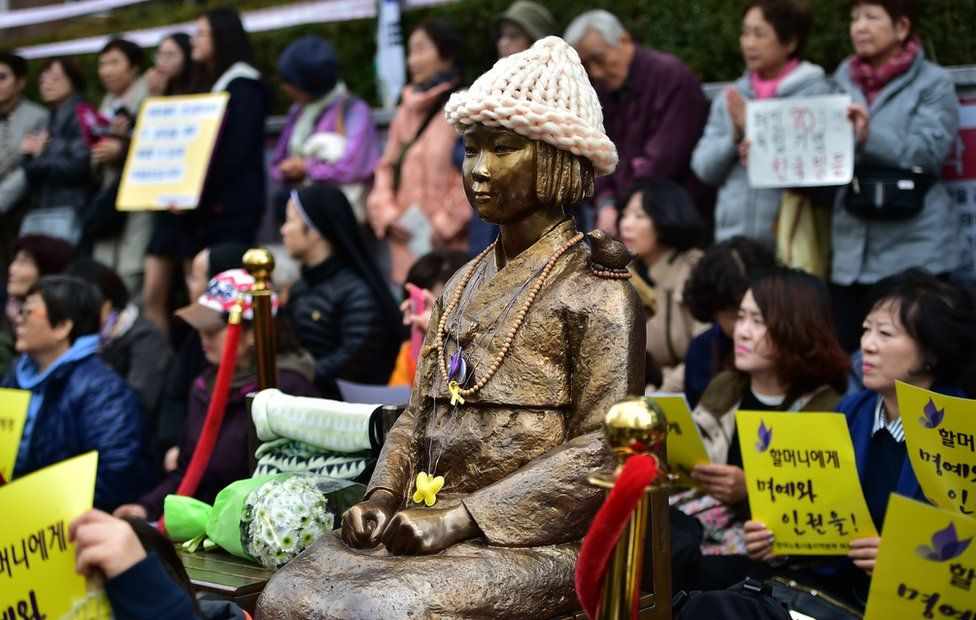
\includegraphics[width = \linewidth]{/Users/mz/Desktop/GitHub/teaching/gv217_conflict_analysis/figs/wk24/fig1.png}
    \end{center}
    \tiny Creator: NG HAN GUAN | Credit: AFP/Getty Image | Copyright: 2006 AFP
\end{frame}

\begin{frame}{Mediation: Some Cases}
    \pause
    \begin{center}
        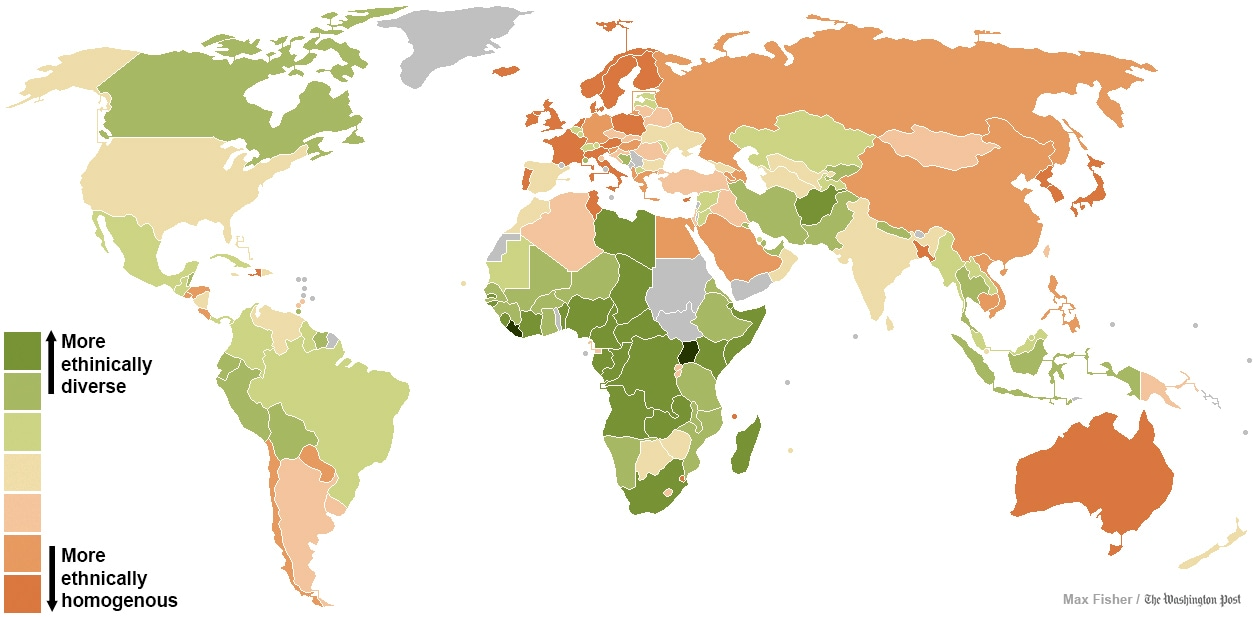
\includegraphics[width = \linewidth]{/Users/mz/Desktop/GitHub/teaching/gv217_conflict_analysis/figs/wk24/fig2.png}
    \end{center}
    \tiny ALEJANDRO ERNESTO, EUROPEAN PRESSPHOTO AGENCY
\end{frame}

\begin{frame}{Mediation: Some Cases}
    \pause
    \begin{center}
        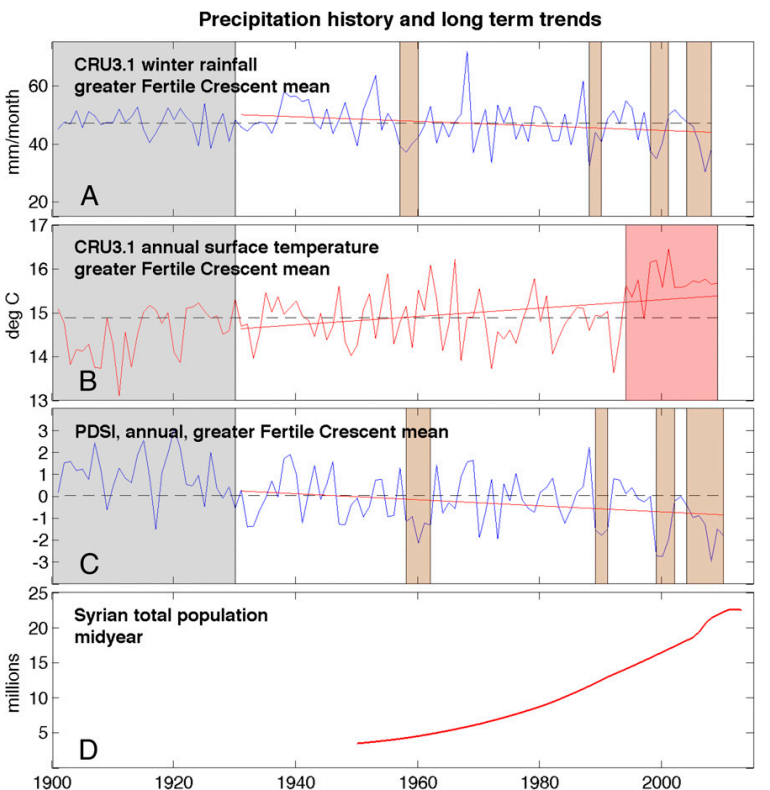
\includegraphics[width = \linewidth]{/Users/mz/Desktop/GitHub/teaching/gv217_conflict_analysis/figs/wk24/fig3.png}
    \end{center}
    \tiny Qatar Ministry of Foreign Affairs (AP)
\end{frame}

\begin{frame}{What Mediators Do?}
    \pause
    \begin{center}
        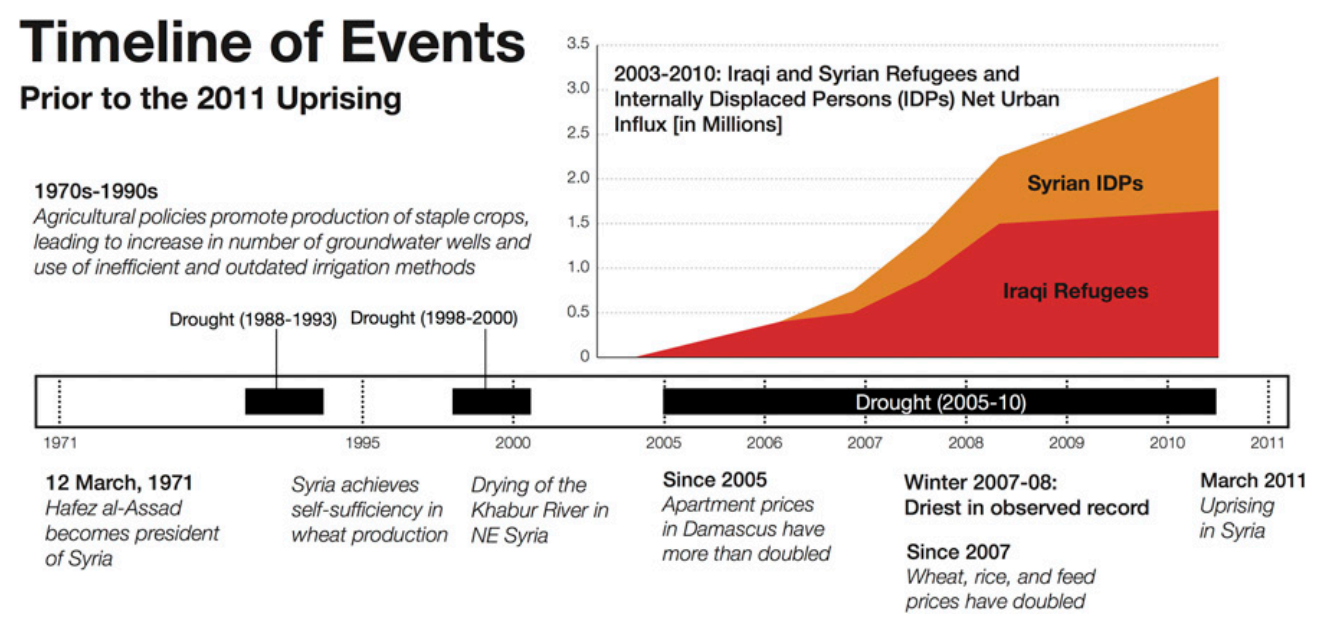
\includegraphics[width = 0.75\linewidth]{/Users/mz/Desktop/GitHub/teaching/gv217_conflict_analysis/figs/wk24/fig4.png}
    \end{center}
    \tiny Table 1, Beardsley et al. (2006)
\end{frame}

\begin{frame}{Why Countries Mediate? Who Are They?}
    \begin{itemize}
        \pause\item Security interest
        \pause\item Economic interest
        \pause\item Political interest---global soft power \& regional influence
        \pause\item Neutral place (politically and geographically)
        \pause\item Safe environment \& reasonable logistics
        \pause\item Fair relationships w both sides
    \end{itemize}
\end{frame}

\begin{frame}{Mediation: Trend}
    \pause
    \begin{center}
        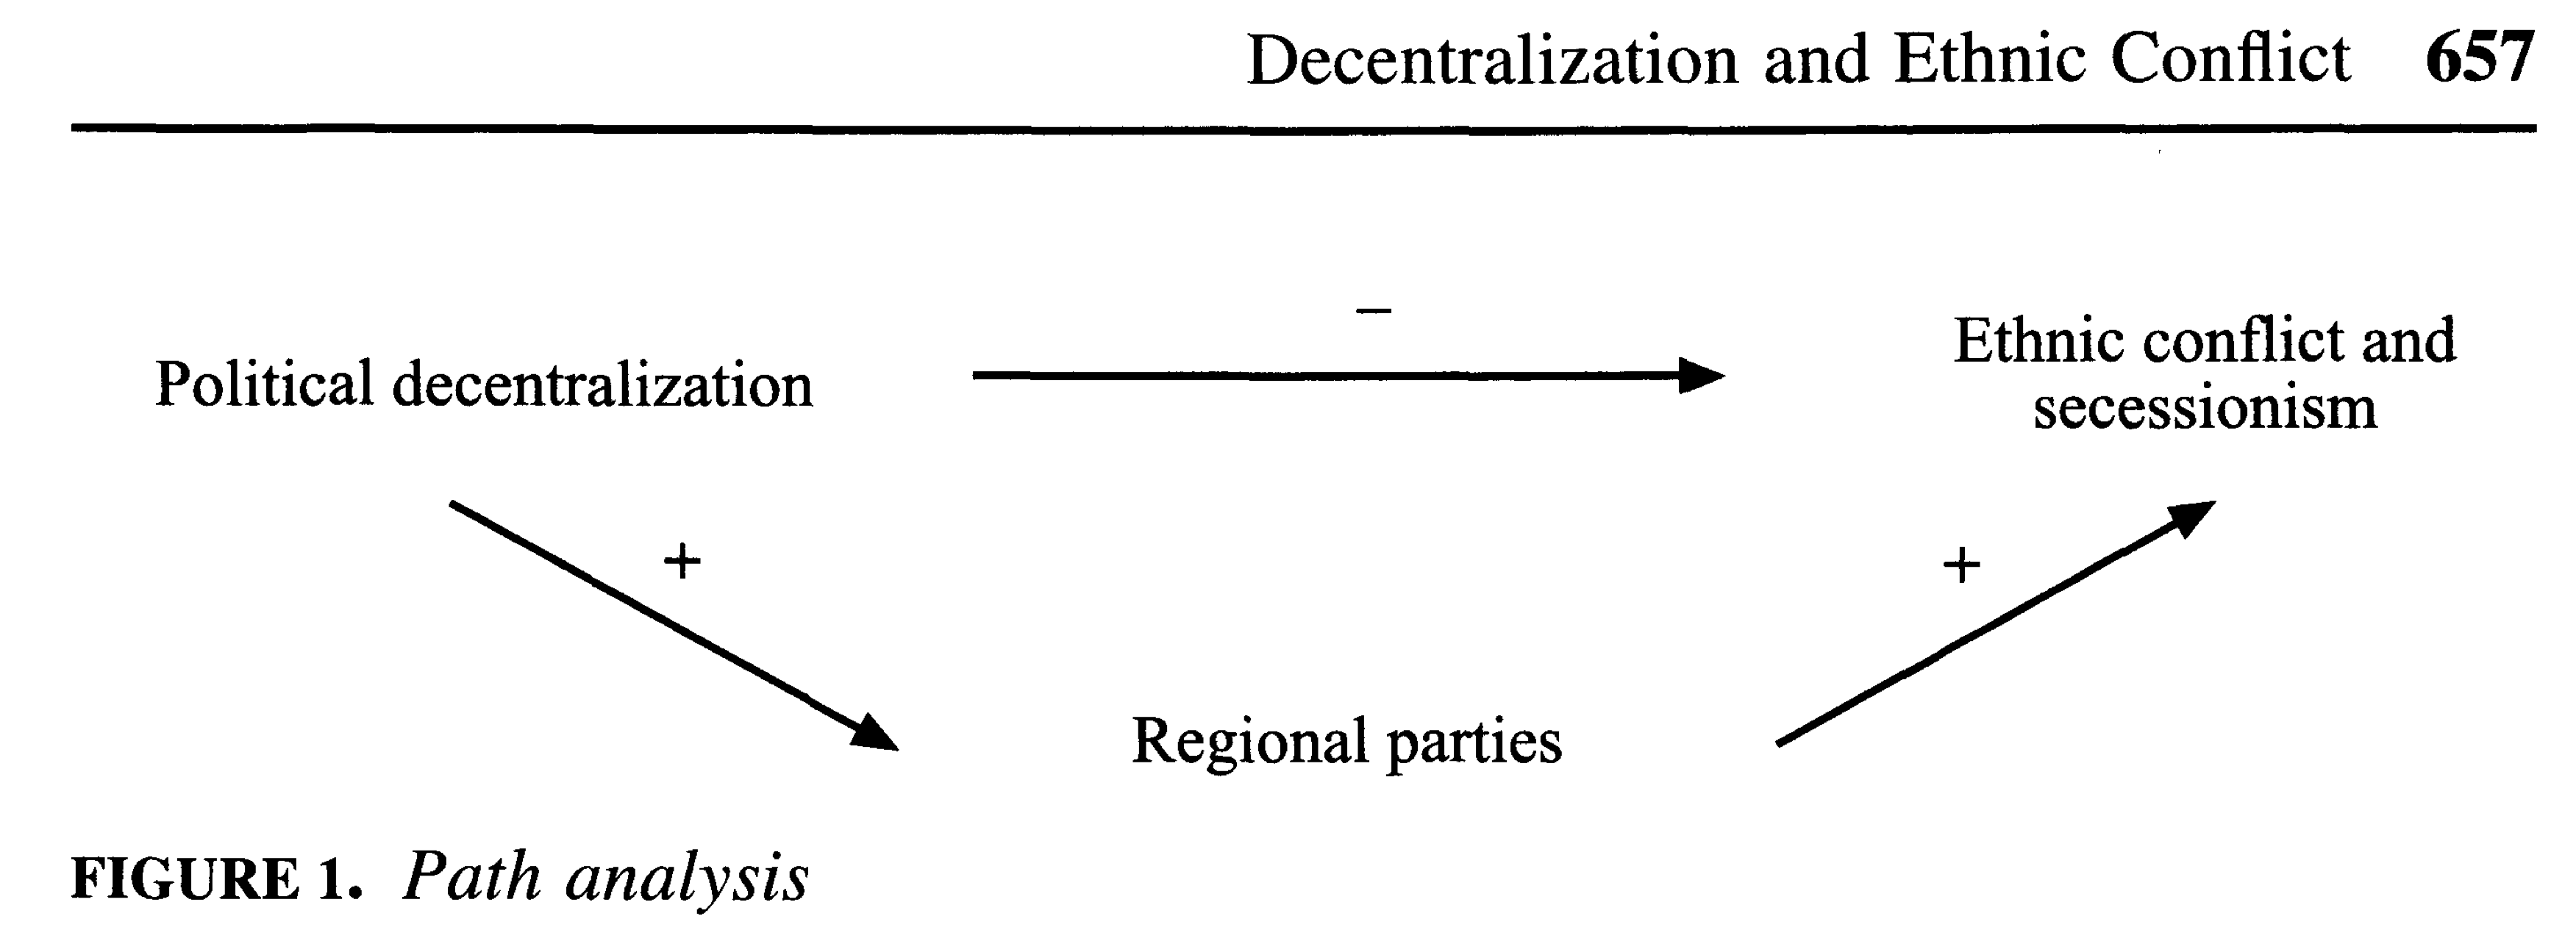
\includegraphics[width = 0.75\linewidth]{/Users/mz/Desktop/GitHub/teaching/gv217_conflict_analysis/figs/wk24/fig5.png}
    \end{center}
    \tiny The ICB Project
\end{frame}

\begin{frame}{Mediation: The ICB Project}
    \pause
    \begin{center}
        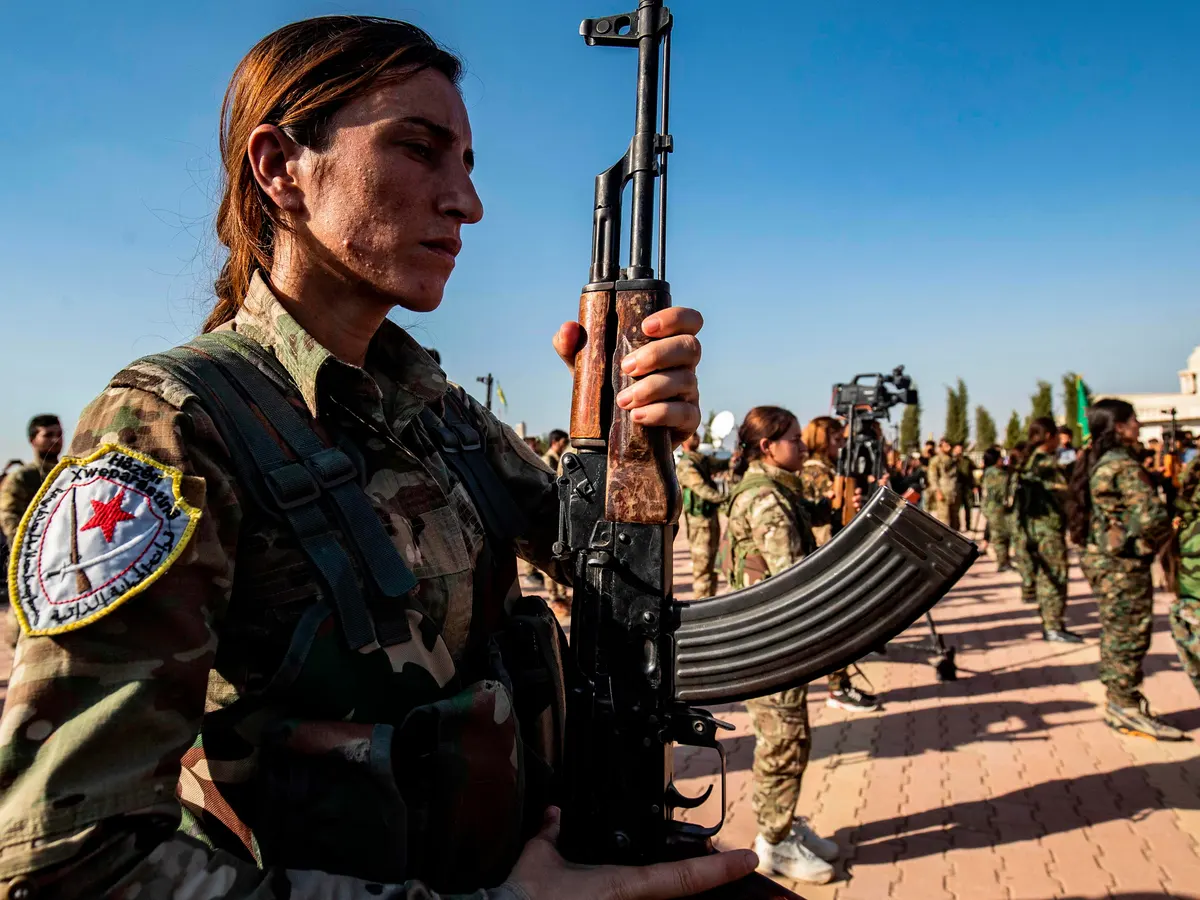
\includegraphics[width = \linewidth]{/Users/mz/Desktop/GitHub/teaching/gv217_conflict_analysis/figs/wk24/fig6.png}
    \end{center}
\end{frame}

\begin{frame}{Conflict Resolution (Hartzell \& Hoodie 2003)}
    Different types of power-sharing
    \begin{itemize}
        \pause\item Political
        \pause\item Economic (wk19)
        \pause\item Territorial
        \pause\item Military (wk19)
        \pause\item Democratization?
    \end{itemize}
    Is there a causation between power-sharing and conflict settlement?
\end{frame}

\end{document}